\documentclass[letterpaper,12pt]{article}
\usepackage{graphicx}
\usepackage[top=1.10in,right=1.2in,bottom=1.4in,left=1.2in]{geometry} 

\frenchspacing  % Removes extra spacing after period.

\usepackage{xfrac}


\usepackage{hyperref}

\usepackage{natbib}
%\usepackage{times}

\usepackage{amsmath}
%\usepackage{hyperref}

\usepackage{color}

\usepackage{pa}

\newcommand{\proglang}{\texttt}
\newcommand{\pkg}{\texttt}


\title{Evaluating measurement invariance in categorical data latent variable models with the  $\da$}

\author{--BLINDED VERSION--}
\date{}

\usepackage{bm}
\newcommand\vm[1]{% Vector or matrix
\bm{\mathrm{#1}}} 

\newcommand{\av}{\vm{a}}
\newcommand{\vech}{\mathrm{vech}\,}
\newcommand{\vecs}{\mathrm{vec}\,}
\newcommand{\param}{\vm{\theta}}
\newcommand{\bpsi}{\vm{\psi}}
\newcommand{\that}{\hat{\vm{\theta}}}
\newcommand{\psat}{\hat{\vm{\psi}}}
\newcommand{\A}{\vm{A}}
\newcommand{\g}{\vm{g}}
\newcommand{\J}{\vm{J}}
\newcommand{\Id}{\vm{I}}
\newcommand{\Ji}{\vm{J}^{-1}}
\newcommand{\PP}{\vm{P}}
\newcommand{\da}{\textrm{{\sc {EPC}}-interest}}

\usepackage{setspace}
\doublespacing

\begin{document}
\maketitle

%Examples of such latent variables include the ideological positions of US senators, countries' Democracy values, and people's (post)materialism. 
%To deal with this problem, it is common to test the null hypothesis of exactly equal measurement and to account for those violations that are encountered, i.e. ``partial measurement invariance''. Several problems with measurement invariance testing have recently led to the introduction of several new approaches. 


\begin{abstract}
Many variables crucial to the social sciences are not directly observed but instead are latent and measured indirectly. When an external variable of interest affects this measurement, estimates of its relationship with the latent variable will then be biased. Such violations of ``measurement invariance'' may, for example, confound true differences across countries in postmaterialism with measurement differences.
To deal with this problem, researchers commonly aim at ``partial measurement invariance'', i.e. to account for those differences that may be present and important. To evaluate this importance directly through sensitivity analysis, the ``EPC-interest''   was recently introduced  for continuous data. However, latent variable models in the social sciences often use categorical data. The current paper therefore extends the EPC-interest to latent variable models for categorical data and demonstrates its use in example analyses of US Senate votes as well as respondent rankings of postmaterialism values in the World Values Study. 

Program inputs and data for the examples discussed in this article are provided in the electronic appendix (\url{http://}[blinded]).
\end{abstract}





\section{Introduction}

\noindent
Latent variable models for categorical data are commonly used in the social and behavioral sciences, and include well-known special cases such as latent class analysis, item response theory (IRT), and ordinal factor analysis. Examples of such analyses include ideological positions of US senators measured by Yea/Nay votes \citep{poole1985spatial}, public tolerance for nonconformity measured by categorical questions in a survey \citep{mccutcheon1985latent}, and  postmaterialism  measured by respondents' rankings of values \citep{inglehart1977silent,moors2007heterogeneity}.

%Examples of latent variable models with categorical data in social science: the ideological positions of US senators, ..., and people's (post)materialism.

Primary scientific interest in latent variable models often focuses on the relationship such latent variables have with external variables. For example, on the polarization of ideology by political party, on education and cohort differences in tolerance, or on cross-country differences in postmaterialism. However, if the measurement of the latent variable differs over values of such external variables,  relationship estimates of interest may be biased \citep{steenkamp_assessing_1998}. Thus, ``measurement invariance'' is needed to estimate such relationships. 

%Relating these variables to external variables is often of interest, for example to Party or year, to ..., and to country or country characteristics such as GDP. But if measurement differs over external variable values the relationship estimate of interest may be wrong.

%by detecting any observed indicators that might violate measurement invariance and accounting for this violation in the model
For this reason, whenever the aim is to compare  values of the latent variable, it is common practice to perform ``measurement invariance testing''  \citep[see][for reviews]{vandenberg2000review,schmitt2008measurement}, a practice also known as  testing for ``differential item functioning'' (DIF) in the IRT literature \citep{Holland:1993aa}. That is, detecting any observed indicators that might violate measurement invariance and accounting for these violations in the model. The aim of measurement invariance testing is to ensure the comparability of latent variable scores over values of an external variable. However, currently existing procedures do not necessarily reach this aim because they do not account for the substantive impact of violations of measurement invariance on the relationship parameters of interest \citep{Oberski:WP:EPC-interest}. 

%This is why people do measurement invariance testing (cites). Particularly, the common approach is to account for those violations of it that are present, partial measurement invariance (cites).

To this end, \citet{Oberski:WP:EPC-interest}  suggested supplementing measurement invariance testing for linear structural equation models with sensitivity analysis. Sensitivity analysis investigates directly the impact of measurement invariance violations on the relationship parameters of interest. It can be performed by fitting many alternative models, with the disadvantage that this process will sometimes be infeasible. \citet{Oberski:WP:EPC-interest} therefore also introduced the EPC-interest, a measure that approximates the change in parameters of interest without the need to fit alternative models. Since  EPC-interest was only introduced for continuous data linear structural equation models, however, it is not applicable to categorical data analyses such as those described above.

%As argued by Oberski (cites), presence is not so relevant but rather importance is, that is, whether measurement invariance affects the conclusions. Suggest to evaluate the robustness of the results of interest to measurmenet invariance assumptions using EPC-interest. EPC-interest estiamtes teh change in the parameter of interest when freeing a measurement invariance restriction. But only for continuous data.

In this paper we therefore extend the EPC-interest approach to measurement invariance testing  to  the case of categorical data latent variable models. The extended measure is evaluated in a small simulation study, and its use demonstrated in two example applications. In the first of these applications the polarization of the 90th US senate is examined by applying an ideal point model; the second application analyzes the rankings of value priorities given by 67,568 WVS respondents in 48 countries. 

%Here for categorical data like the data mentioned above. Need to account for dependencies between parameters to do with the same category.

\bigskip
Section \ref{sec:invariance} explains categorical data latent variable models  and the problem of measurement invariance. The EPC-interest is introduced in Section \ref{sec:epc-interest} as an approximation to the sensitivity analysis approach to measurement invariance testing and a small simulation study evaluates the approximation in Section \ref{sec:simulation}. Sections \ref{sec:rollcall} and \ref{sec:WVS} then elaborate the two example applications, while Section \ref{sec:discussion} concludes. 


\section{Measurement invariance in categorical data}
\label{sec:invariance}
\subsection{The problem of measurement invariance}

Many important variables in the social sciences are not or cannot be directly observed, but are instead latent  \citep{bollen2002latent} and measured using a vector of multiple indicators, $\mathbf{y}$, say. This measurement of the latent variable $x$ is defined by a ``measurement model'',
\begin{equation}
	p(\mathbf{y} | x).
		\label{eq:measurement-model}
\end{equation}
The latent $x$ variable could, for example, be a ``random effect'', a person's unobserved utility for a choice, a general attitude, or a variable measured with error such as voter turnout.
Often the measurement model in Equation \ref{eq:measurement-model} is not, however, of primary interest to the researcher, but rather  the relationship between the latent variable and some covariate vector $\mathbf{z}$ is, i.e. the ``structural model'',
\begin{equation} 
	p(x | \mathbf{z}).
		\label{eq:structural-model}
\end{equation}
Figure \ref{fig:LVM} shows this relationship as an arrow between the observed covariate $\mathbf{z}$ and latent variable $x$.
For example, $\mathbf{z}$ could contain a set of dummy variables indicating a respondent's country or gender, so that Equation \ref{eq:structural-model} simply compares values of $x$ across countries or genders. Alternatively, interest could focus on the influence of continuous covariates such as GDP or age on the latent $x$. Of course, the problem is that $x$ is not observed, but only $\mathbf{y}$ and $\mathbf{z}$ are. 

\begin{figure}\centering
	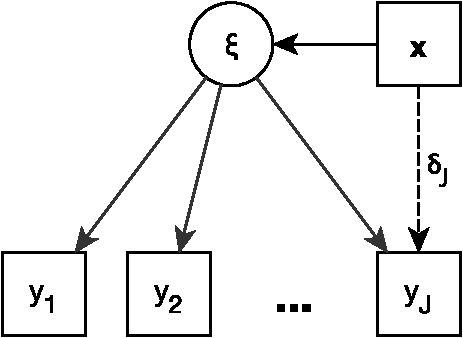
\includegraphics[width=.4\textwidth]{figures/LVM}
	\caption{Graph of a latent variable model. The latent variable $x$ is shown in a circle to indicate that it is unobserved. }
	\label{fig:LVM}
\end{figure}

Latent variable models generally attack this problem by making two key assumptions about how $x$ is measured \citep{skrondal2004generalized}. The first assumption is necessary to identify the measurement model. It states that, given the latent variable, the indicators $y_j$ are ``locally independent'': $
%\begin{equation}
		p(\mathbf{y} | x) = \prod_{j \in \{1..J\}} p(y_j | x),
%		\label{eq:local-independence}
%\end{equation} 
$ where $J$ is the number of indicators use to measure $x$; typically $J$ will be at least three. In Figure \ref{fig:LVM}, the  absence of relationships among the observed variables except those due to their common cause $x$ implies local independence.
%The local independence assumption is common to all multiple indicator latent variable models and not specific to the issue of relating the covariate to the latent variable. 

The second assumption is necessary to identify the structural model. It states that, while the latent variable may depend on the covariate, its \emph{measurement} should not, i.e. the indictors should be ``measurement invariant'':
\begin{equation}
	p(y_j | x, \mathbf{z}) = p(y_j | x).
	\label{eq:no-dif}
\end{equation}
When Equation \ref{eq:no-dif} holds for \emph{all} $J$ indicators this is called ``full measurement invariance'' \citep{meredith1993measurement}. 
A violation of  measurement invariance is sometimes termed ``differential item functioning'' (DIF), since the ``items'' $y_j$ have differing conditional probability distributions given $x$ for differing values of $\mathbf{z}$ \citep{mellenbergh1989item}.
Intuitively, measurement invariance is necessary to identify the structural model of Equation \ref{eq:structural-model} because if all indicators are caused by both $x$ and $\mathbf{z}$, then there is no way of knowing whether an observed indicator difference  over values of the covariate is due to a covariate effect on  $x$ or to a difference over the covariate in the way $x$ is measured. For example, when comparing countries, an observed cross-country difference in anti-immigrant attitudes might be a substantive difference or it might equally well be explained as differing answer tendencies over countries. 
%Since the same is true for all the other indicators, there is just no way of separating effects on indicators from effects on the latent variable: the structural model is therefore unidentifiable.  Full measurement invariance thus guarantees that $x$ can indeed be compared across values of the covariates.

This identification problem only occurs, however, when there are no measurement invariant indicators at all. A single invariant indicator can disentangle measurement from substantive differences in the other, non-invariant, indicators. Full measurement invariance is therefore not necessary to identify the structural model, but ``partial measurement invariance'' is \citep{byrne1989testing}. The standard practice is to search for non-invariant indicators and either remove them or parameterize their differential functioning \citep{Holland:1993aa}. 
A common way of doing so when the observed variables are categorical with $K$ categories is a logistic regression, 
\begin{equation}
	P(Y_j = k) = \frac{\exp(\tau_{jk} + \lambda_{jk} x + \delta_{jk} \mathbf{z})}{\sum_{m \in \{1..K\}} \exp(\tau_{jm} + \lambda_{jm} x + \delta_{jm} \mathbf{z})},
	\label{eq:logistic-dif}
\end{equation}
\citep{mellenbergh1989item,kankaras2010testing}, where some restriction is imposed on the parameters for identification purposes such as ``effect coding'', $\sum_k \tau_{jk} = \sum_k \lambda_{jk} =\sum_k \delta_{jk} = 0$, or dummy coding, $\tau_{j1} = \lambda_{j1} = \delta_{j1} = 0$. 
It can be seen in Equation \ref{eq:logistic-dif} that setting $\delta_{jk} = 0$ corresponds to measurement invariance\footnote{An interaction term $\delta_{jk}^* \mathbf{z}x$ could be added to Equation \ref{eq:logistic-dif} but has been omitted for clarity.}. This means that it is possible to estimate a model in which $\delta_{jk} \neq 0$ for \emph{some} indicators, while $\delta_{jk}$ is kept at zero, i.e. partially measurement invariant, for others. 
Figure \ref{fig:LVM} shows this possible direct effect from covariate to indicator as a dashed arrow. 

\subsection{Existing solutions}

In short, some form of measurement invariance is needed to estimate the structural model of interest: deciding which form, that is, selecting a model, is therefore crucial. Currently, there are broadly three existing approaches to doing so:
\begin{enumerate}
	\item Selecting one indicator as the reference indicator or ``anchor item'' \emph{a priori};
	\item Imposing a strong prior on the differential functioning parameters \citep{muthen2012bayesian};
	\item Testing the null hypothesis of full measurement invariance \citep{steenkamp_assessing_1998,french2006confirmatory} or partial measurement invariance, in which violations of invariance are freed  \citep{byrne1989testing,saris2009testing}.
\end{enumerate}

\emph{A priori} reference indicators are often selected implicitly, for example by setting one loading to unity in multiple group CFA. A recent extension to this approach, the ``alignment method'', was suggested by \citet{muthen2014alignment}. When the researcher is not certain that the ``reference indicator'' is indeed invariant, however, it is impossible to select it based on the data \citep{hancock2009tenuousness}. The Bayesian approach suggested by \citet{muthen2012bayesian} has the distinct advantage that, when the prior has been chosen aptly, the data can determine which indicators should be more or less invariant -- hence the term ``approximate measurement invariance'' \citep[see also][]{schoot2013facing}. However, if the prior is not chosen adequately, for instance if it is too strong or too weak, bias in the parameters of interest may still occur. At current this remains a topic for future study, although the approach is promising. Finally, it is common to test for full or partial measurement invariance using various fit measures available for this purpose \citep{byrne1989testing,hu1998fit,cheung2002evaluating,chen2007sensitivity,saris2009testing}. However, this approach has recently been shown to have an unfortunate disadvantage: when a violation is detected, it need not have seriously affected the parameter of interest, and when an invariance model is selected, substantial bias in the parameter of interest may still remain \citep{Oberski:WP:EPC-interest}. In short, while measurement invariance is an important assumption in latent variable modeling, the existing methods do not directly account for the effect that violations of this assumption have on the parameters of interest.

To complement measurement invariance testing, the 
 EPC-interest was therefore recently introduced by \citet{Oberski:WP:EPC-interest} for continuous data structural equation models. The EPC-interest assesses what would happen if a particular possible direct effect were freed. Rather than assessing the size of this direct effect itself, however, it assesses its impact on the parameter of interest. However, this measure is only available for continuous data, whereas many important measures of latent variables in the social sciences are categorical. Examples include the votes (Yea/Nay) of senators indicating their ideology, how respondents rank their value priorities (1 through 4), or answers (correct/incorrect) to political knowledge questions. The following section therefore extends the EPC-interest to the case of categorical indicators.

\subsection{EPC-interest}
\label{sec:epc-interest}

The ``$\da$'' estimates the change in a free parameter estimate of the model that one can expect to observe if a particular restriction were freed. It is therefore a method of sensitivity analysis. However, the researcher is not forced to estimate all possible alternative models, but can evaluate the sensitivity of the results after fitting the restrictive full invariance model. 
The $\da{}$ is based on the work of \citet{saris_detection_1987}, who introduced the expected parameter change in a fixed parameter for linear structural equation models (SEM), and \citet{bentler1993some}, who introduced the expected parameter change in a free parameter after freeing a fixed parameter for SEM. It was applied to invariance testing with continuous data by \citet{Oberski:WP:EPC-interest}.

In models for categorical data, the EPC-interest can be derived, as shown below and in the Appendix, by applying general results of maximum likelihood analysis. An additional problem with categorical data, however, is that there are usually sets of parameters relating to particular variables. For example, in Equation \ref{eq:logistic-dif}, there will be $K$ ``loadings'' $\lambda_{jk}$, $K$ ``intercepts'' $\tau_{jk}$,  $K$ ``direct effects'' $\delta_{jk}$, and, if present, $K$ ``interaction effects'' $\delta^*_{jk}$ for each variable. This principle may be familiar from ANOVA: when an ANOVA term corresponds to a categorical variable, it will have several parameters that are considered simultaneously in the analysis. These parameters will, moreover, be strongly dependent on one another, so that the impact of freeing one of them cannot be seen separately from the impact of freeing another parameter relating to the same variable. 

For this reason, when extending EPC-interest to the categorical case, it also becomes necessary to allow for the consideration of \emph{sets} of parameters to free rather than just investigating the effect of single restrictions. This requires a multivariate EPC-interest, rather than the univariate one in use so far. Furthermore, while for linear SEM estimates the necessary closed-form expected gradients and hessians are available \citep{Oberski:WP:EPC-interest}, in order to extend the EPC-interest to categorical data models, which differ considerably in the form these quantities take, we will take a more general approach here.

%For example, in structural equation models with ordered categorical indicators \citep{muthen_general_1984}, we would recommend considering the effect of freeing all thresholds as a set, rather than considering the effect of the threshold for each category separately. By the model's definition, such parameters are strongly dependent. 

In deriving the EPC-interest, the key concept is considering the likelihood not only as a function of the free parameters of the model, but also as a function of the parameters that are fixed to obtain the full invariance model. Collecting the free parameters in a vector $\param$ and the fixed parameters in a vector $\bpsi$, we assume the likelihood can be written as an explicit function of both sets of parameters, $L(\param, \bpsi)$.  The maximum-likelihood estimates $\that$ of the free parameters can then be seen as obtained under the full invariance model that sets $\bpsi=0$, i.e. $\that = \arg\max_{\param} L(\param, \bpsi = 0)$. Further, define the parameters of substantive interest as $\vm{\pi} := \vm{P} \param$, where $\vm{P}$ is typically a logical (0/1) selection matrix, although any linear function of the free parameters $\param$ may be taken. 
Interest then focuses on the likely value these free parameters $\vm{\pi}$ would take if the fixed $\bpsi$ parameters were freed in an alternative model, $\hat{\vm{\pi}}_a = \vm{P} \arg\max_{\param, \bpsi} L(\param, \bpsi)$. 

We now show how these changes in the parameters of interest as a consequence of freeing the fixed parameters $\bpsi$ can be estimated without fitting the alternative model. Let the Hessian $\hat{\vm{H}}_{\vm{a}\vm{b}}$ be the matrix of second derivatives of the likelihood with respect to vectors $\vm{a}$ and $\vm{b}$, evaluated at the maximum likelihood solution of the full invariance model, $\hat{\vm{H}}_{\vm{a}\vm{b}} := (\partial^2 L /\partial \vm{a} \partial \vm{b}^\prime)|_{\param=\that}$. 
The expected change in the parameters of interest is then measured by the $\da$, 
\begin{equation}
\da = \hat{\vm{\pi}}_a - \hat{\vm{\pi}} = \vm{P}
%	\left( \frac{\partial^2 L(\param, \bpsi)}{\partial (\param, \bpsi)^\prime \partial (\param, \bpsi)} \right)^{-1}
%		\vm{D}^{-1} \hat{\vm{H}}_{\param\bpsi}^\prime \hat{\vm{H}}^{-1}_{\param\param}
\hat{\vm{H}}^{-1}_{\param\param} \hat{\vm{H}}_{\param\bpsi}\vm{D}^{-1}
		\left[ \left.\frac{\partial L(\param, \bpsi)}{\partial \bpsi}\right|_{\param = \that} \right] +	
		O(\vm{\delta}^\prime\vm{\delta}),
		\label{eq:epc-interest}
\end{equation}
where $\vm{D}:= \hat{\vm{H}}_{\bpsi\bpsi} - \hat{\vm{H}}_{\param\bpsi}^\prime \hat{\vm{H}}^{-1}_{\param\param} \hat{\vm{H}}_{\param\bpsi}$ and the deviation from the true values is $\vm{\delta}:= \vm{\vartheta} - \hat{\vm{\vartheta}}$, with $\vm{\vartheta}$ collecting the free and fixed parameters in a vector, $\vm{\vartheta}:= (\param^\prime, \bpsi^\prime)^\prime$. Note that, apart from the order of approximation term $O(\vm{\delta}^\prime \vm{\delta})$,  Equation \ref{eq:epc-interest} contains only terms that can be calculated after fitting the invariance model.
%(Relevant derivatives for the special case of the multilevel latent class model are given in Appendix \ref{app:derivatives}.)
 Thus, it is not necessary to fit the alternative model to obtain the $\da{}$.

In the structural equation modeling literature, the expected change in the fixed parameters $\bpsi$  is commonly found and implemented in standard SEM software. This measure is commonly know as the ``EPC'', but to avoid confusion we term it ``EPC-self'' here. The EPC-self and $\da{}$ both consider the impact of freeing restrictions, but differ in the target of this impact: the EPC-self evaluates the impact on the restriction itself, whereas the $\da{}$ evaluates the impact on the parameters of interest. In spite of these differences, the two measures are related: this can be seen by recognizing that $- \vm{D}^{-1}
		\left[ \left.\frac{\partial L(\param, \bpsi)}{\partial \bpsi}\right|_{\param = \that} \right] = \text{EPC-self} \approx \bpsi - \hat{\bpsi}$ so that, from Equation \ref{eq:epc-interest}, 
\begin{equation}
\da=- \vm{P} \hat{\vm{H}}^{-1}_{\param\param} \hat{\vm{H}}_{\param\bpsi} \,\text{EPC-self} \approx
- \vm{P} \hat{\vm{H}}^{-1}_{\param\param} \hat{\vm{H}}_{\param\bpsi} \left( \bpsi - \hat{\bpsi}\right)
\end{equation}
Furthermore, since $\hat{\bpsi}$ and $\hat{\param}$ are implicitly related by the fact that they are both solutions to the equation $\partial L / \partial \vm\vartheta = \vm{0}$, invoking the implicit function theorem yields $- \hat{\vm{H}}^{-1}_{\param\param} \hat{\vm{H}}_{\param\bpsi}  = \partial \param / \partial \bpsi^\prime$, so that 
\begin{equation}
	\da = \vm{P} \left( \frac{\partial \param} {\partial \bpsi^\prime} \right) \left( \bpsi - \hat{\bpsi}\right),
	\label{eq:epc-linear}
\end{equation}
that is, the $\da{}$ can be seen simply as the coefficient of a linear approximation to the relationship between the free and fixed parameters, multiplied by the change in the fixed parameters. This demonstrates the difference with the sensitivity analysis approach common in econometrics \citep[p. 168]{magnus2007local} in which only $\partial \param / \partial \bpsi^\prime$ is considered: the $\da{}$ combines both the direction ($\partial \param / \partial \bpsi^\prime$) and the magnitude ($ \bpsi - \hat{\bpsi}$) of the misspecification.


The accuracy of the approximation of the $\da{}$ as a measure of the change in the parameters of interest is reflected in the order of approximation term, $O(\vm{\delta}^\prime\vm{\delta})$. It can be seen that this accuracy is quadratic in the overall change in parameters, so that the approximation can be expected to work best when the misspecifications are not ``too large''. This result corresponds to results on the score test (``modification index'') and ``EPC-self'' in the literature on structural equation modeling, which can be shown to be exact under a ``sequence of local alternatives'', i.e. when $\vm{\vartheta} = \lim_{n\rightarrow\infty} \hat{\vm{\vartheta}} + n^{-\frac{1}{2}}\vm{\delta}$ \citep[p. 135]{satorra1989alternative}.
It is important to note here that $\vm{\delta}$ is the deviation from the ``true'' value of $\vm{\vartheta}$, rather than the deviation from the limit of the parameter estimates under the alternative model. Therefore another view on the accuracy is that it will be better when the alternative model is not strongly misspecified. For this reason it is also important to consider freeing sets of very strongly related parameters simultaneously, since a change in one of them will then imply a change in the others, and, consequently, a misspecified alternative model.

\subsection{Small simulation study}
\label{sec:simulation}

To demonstrate the extent of the approximation bias in the EPC-interest, we performed a small simulation study. In this study, we specified a latent variable model for four binary indicators:
$
	P(Y_j = 1 | x) = [1 + \exp(-x)]^{-1},
$
with $j \in \{2,3,4\}$, and structural model
$
	x = \gamma z + \epsilon
$
with $\gamma = 1$ and $\epsilon \sim N(0, 1)$. We then introduced a violation of measurement invariance for the first indicator,
$
	P(Y_1 = 1 | x) = [1 + \exp(-x - \delta z)]^{-1}.
$
Nine conditions varied sample size, $n \in \{250, 500, 1000\}$, and the size of the invariance violation:  $\delta = $ 0 (no violation), 0.5 (moderate), or 1 (extreme). 
Data were generated using R 3.1.2 and analyzed using Latent GOLD 5.0.0.14161. 

\begin{table}\begin{small}
\begin{tabular}{lrrrrrrrrrrrr}
\hline
$n$	& \multicolumn{3}{c}{250} && \multicolumn{3}{c}{500} && \multicolumn{3}{c}{1000} \\
	\cline{2-4}	\cline{6-8} 	\cline{10-12}
True $\delta$	&   0	& 0.5	& 1	&& 0	& 0.5	& 1	&& 0	& 0.5	& 1\\
	\hline
	Est. $\hat{\gamma}$	& 1.010	& 1.151	& 1.353	&& 0.980	& 1.152	& 1.330	&& 1.013	& 1.163	& 1.327\\
	Bias $\hat{\gamma}$ & -0.010	& -0.151	& -0.353	& 	& 0.020	& -0.152	& -0.330	& 	& -0.013	& -0.163	& -0.327\\

	EPC-int.	& 0.003	& -0.166	& -0.494&	& -0.001	& -0.180	& -0.486&	& 0.004	& -0.182	& -0.448\\
\hline
\end{tabular}
\caption{Simulation study of EPC-interest. Shown is the average point estimate for the $\gamma$ parameter of interest under full measurement invariance (``Est''), its difference from the true value $\gamma=1$ (``Bias''), and the average EPC-interest.}
\label{tab:simulation}
\end{small}\end{table}

The results over 200 samples are shown in Table \ref{tab:simulation}. The first two rows  show the average point estimate of the parameter of interest $\hat{\gamma}$, and its deviation from the true value $\gamma = 1$, respectively. It can be seen that a modest violation $\delta = 0.5$ still has a substantively important impact on bias. Under this condition, the amount of bias is reasonably well approximated by the EPC-interest, which has average values close to the true bias. When the violation is extreme, however, the approximation causes the EPC-interest to somewhat overestimate the bias: for example, in the last column of the table the true bias is -0.327 but EPC-interest estimates it at about -0.448. The bias does not appear to be strongly affected by the sample size, demonstrating the asymptotic approximation results above. 


Overall, the results of this very limited simulation study demonstrate the analytic results discussed above. As expected, for very large violations of invariance the EPC-interest will overestimate the bias caused somewhat. In these cases, the EPC-interest is still a useful guide but the researcher may wish to verify that after freeing the violation in question, the results of interest do indeed change substantially. Alternatively, where this is feasible, one may also resort to estimating all alternative models and examining the results. In other conditions, the EPC-interest performs as expected: when there is no bias, it estimates zero on average, and when there is moderate bias in the parameter of interest, EPC-interest approximates this bias adequately. 


\section{Example application \#1: 90th US Senate roll call data}
\label{sec:rollcall}

To exemplify the use of the EPC-interest using a relatively simple latent variable model with categorical variables that is well-known in political science, we estimate an ideal point model on roll call data for senators in the 90th US Senate, which met from 1967 to 1969 during the Lyndon B. Johnson Administration. 

The probability that senator $i$ votes ``Yea'' on motion $j$ is modeled as a logistic regression on the motion's (unobserved) utility, 
\begin{equation}
	P(\text{``Yea'' on motion } j | x_i) = [1 + \exp(-\beta_j u_{ij})]^{-1},
	\label{eq:vote-nodif}
\end{equation}
where the utility $u_{ij}$ of the motion to that senator is simply the Euclidean distance between the senator's position $x_i$ and the motion's position $\tau_j$,
\begin{equation}
	u_{ij} = (x_{i} - \tau_{j})^2.
\end{equation}
This model is equivalent to the well-known unidimensional \citet{poole1985spatial} (W-NOMINATE) model. The latent value $x_i$ is known  as an ``ideal point''. 

The Poole-Rosenthal model can be extended to incorporate covariates that predict the latent variable $x_i$, for example using the party of the senator as a predictor: 
\begin{equation}
	x_i = \alpha + \gamma \cdot \text{Party} + \epsilon_i.
	\label{eq:party-dimension}
\end{equation}
Using party (Democratic or Republican) as a predictor allows the researcher to see how strongly  party membership relates to  senators' ideological positions, which ultimately influences their votes. A higher value of $\gamma$ thus indicates more ideological homogeneity  within parties in the Senate: we therefore call $\gamma$ the ``polarization coefficient''.  

The usual choice $\epsilon_i \sim \text{Normal}(0, \sigma^2)$  leads to a quadratic structural equation model (SEM) for categorical data, or, equivalently, a quadratic 2PL IRT model with a covariate \citep{rabe2004generalized}. Alternatively, the distribution of $x$ can be estimated from the data by choosing some number $K$ of categories for $x$ (``latent classes'') and modeling the probability of belong to class $k$ as an ordered multinomial regression,
\begin{equation}
	P(x_i = k | \text{Party}) = \frac{\exp(\alpha_k + \gamma \cdot x^{(k)} \cdot \text{Party})}
		{\sum^{K}_{m=1} \exp(\alpha_m + \gamma \cdot x^{(m)} \cdot \text{Party})},
\end{equation}
where $x^{(k)}$ is a latent score assigned to the $k$-th category of $x$. For this arbitrary choice of latent scale, we choose $x^{(k)}$ to go from 0 to 1 in equally spaced intervals \citep[following][]{vermunt2013technical}. The latent category intercepts $\alpha_k$ allow the distribution of the latent dimension to be freely estimated rather than assumed Normal. This leads to the ``latent class factor model'' \citep{vermunt_factor_2004}.


%In familiar techniques such as W-NOMINATE or Optimal Classification Roll Call Scaling \citep{Poole:2005aa}, investigating the relationship of the latent dimension $x_i$ with external variables is often accomplished by first estimating the ideal point estimates $\hat{x}_i$ and then correlating or plotting these values with the covariate. The current formulation 	\label{eq:party-dimension} attains the same goal in one step, with the possible advantage that measurement error in the ideal point estimates is accounted for in the estimation of the polarization coefficient of interest $\gamma$.

A possible problem when using ideal point models to investigate polarization is that it is assumed that this polarization is the same on all motions the Senate votes on. If there is some motion on which the votes of senators from the same party are significantly more tight-knitted than usual, there will be an effect of Party over and above that of the senator's utility for this motion. A vote model with a direct covariate effect,
\begin{equation}
		P(\text{``Yea'' on motion } j | x_i) = [1 + \exp(-\beta_j u_{ij} - \delta_j \cdot\text{Party})]^{-1},
	\label{eq:vote-dif}
\end{equation}
then replaces Equation \ref{eq:vote-nodif}. In other words, the usual ideal point model assumes measurement invariance with respect to the covariate, an assumption that can be expressed as $\delta_j=0$. Where such direct effects do exist they are relevant to the investigation of polarization insofar as ignoring them biases the estimate of the Senate's overall polarization. Thus, we investigate whether the assumption of measurement invariance $\delta_j=0$  seriously affects the estimate of interest $\hat{\gamma}$ using the EPC-interest.

Maximum likelihood estimates of the parameters were obtained using the software Latent GOLD, taking $K=4$ and the first 20 motions introduced in the 90th Senate as an example. The model appears to fit the data well, with an $L^2$ bootstrapped $p$-value of $0.14$, The factor scores $\hat{x}_i$ obtained from this simple model correlated highly (0.79) with those obtained from W-NOMINATE \citep{poole2008scaling} and from Optimal Classification Roll Call Scaling \citep[0.81;][]{poole2012oc}. Based on the full invariance model, the polarization coefficient $\hat{\gamma}$ was estimated at $4.164$ (s.e. 1.3077). Since $\gamma$ is a logistic regression coefficient,  a Republican senator has about four times higher odds of being one category above a Democratic senator than of being in the same category\footnote{Because there are four $x$ categories scored $\{0, \sfrac{1}{3}, \sfrac{2}{3}, 1\}$, the odds are $\exp(\hat{\gamma}/3)\approx4$.}. There was therefore considerable polarization in the 90th Senate. 

However, violations of measurement invariance could conceivably bias this conclusion. To investigate this, Figure \ref{fig:epc-interest} plots the EPC-interest values of freeing the direct effects $\delta_j$ on the parameter estimate of interest $\hat{\gamma}$. Each number in Figure \ref{fig:epc-interest} corresponds to a motion number introduced in the Senate. The vertical axis, labeled ``EPC-interest'', estimates the change from the current estimate ($\hat{\gamma}=4.164$) under full measurement invariance that one can expect to observe in $\hat{\gamma}$ when freeing the direct effect of Party for that motion. 
The horizontal axis shows the $p$-value for the null hypothesis that the corresponding $\delta_j = 0$, adjusted for false discovery rate \citep{benjamini1995controlling}. The idea behind plotting both of these quantities at the same time is that the researcher will likely be interested in violations of measurement invariance that are both statistically and substantively significant \citep{saris2009testing}.

\begin{figure}\centering
\includegraphics[width=.8\textwidth]{../outputs/EPC-interest.pdf}
\caption{The effect of twenty measurement invariance assumptions on the polarization parameter of interest $\gamma$, plotted against the p-values for each violation.}
\label{fig:epc-interest}
\end{figure}

Figure \ref{fig:epc-interest} shows that, of the statistically significant violations of measurement invariance, motion \#03 violates measurement invariance in a manner that augments the estimated polarization (EPC-interest is positive). Motions \#04 and \#13, violate measurement invariance in an approximately opposite manner (EPC-interests are negative). However, motion \#20, clearly stands out as an important violation of measurement invariance.
After introducing the direct effect of party on voting ``Yea'' to Motion \#20 (freeing $\delta_{20}$), no other measurement invariance violations are statistically significant (all false discovery rate-adjusted $p$-values $\geq 0.05$). Thus, it seems that Motion \#20 (HR4573, which increased the public debt limit) was an issue on which the ranks were closed more than usual. Indeed, the 1967 CQ Almanac\footnote{\url{http://library.cqpress.com/cqalmanac/document.php?id=cqal67-1314297}} specifically reports on this motion, remarking that ``Republicans launched their first major attacks in the 90th Congress on the Administration's fiscal policies'', with no Republicans voting in favor. 

After adjusting for this event, the polarization coefficient is estimated at 3.422 (s.e. 1.0630): the tight-knittedness between party membership and voting pattern is therefore somewhat loosened, but still strong.  The partial invariance model after accounting for this one violation becomes acceptable, in  the sense that those violations that are present do not substantially change the results of interest regarding polarization. The model fit the data well with an $L^2$ bootstrapped $p$-value of $0.11$. Its BIC (1379) indicates an improvement over that of the full invariance model (1405).  Overall, the difference between the fully and partially invariant models are modest. Figure \ref{fig:ideal-points} shows the effect of freeing $\delta_{20}$ on the ``ideal point'' estimates, i.e. the latent variable estimates $\hat{x}_i$. 

\begin{figure}\centering
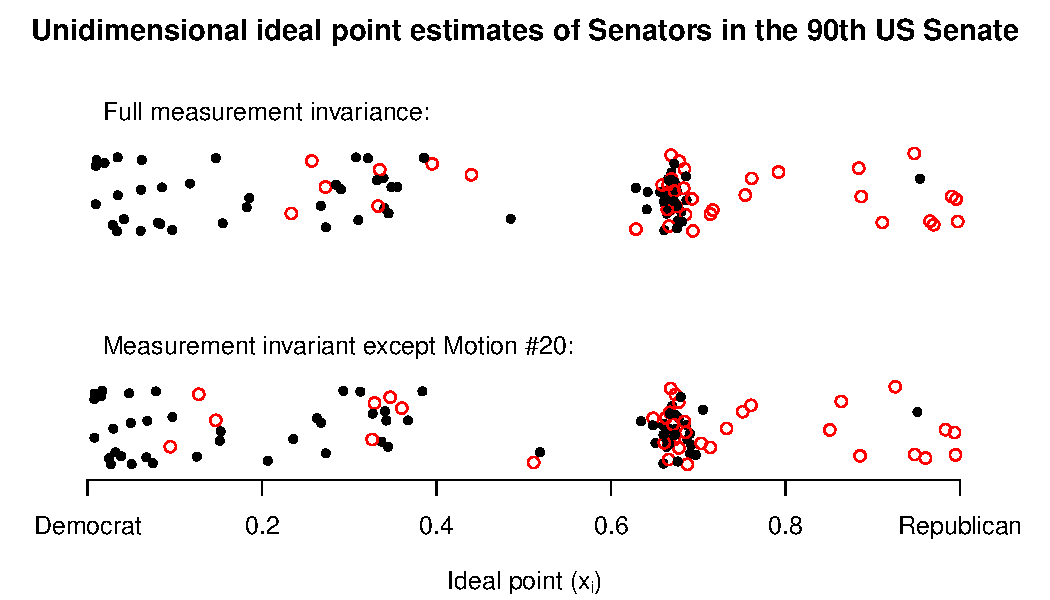
\includegraphics[width=.9\textwidth]{../outputs/ideal-points.pdf}
\caption{Posterior point estimates of the latent variable ``ideal point'' score $\hat{x}_i$ for all senators (points), jittered vertically for visual clarity. Black points are Democrats, red circles Republicans. Top: estimates under the fully invariant model; Bottom: estimates allowing for the direct effect $\delta_{20}\neq0$.}
\label{fig:ideal-points}
\end{figure}

The top part of Figure \ref{fig:ideal-points} shows the ideal point estimates under the full invariance model. These estimates range from zero to one; since Democrats, shown as black dots, are predominantly on the lower side of the scale, zero has been labeled ``Democrat'' and the score 1 has been labeled ``Republican'', since most Republicans (red circles) can be found here. To make the points more visible, they have been jittered randomly in the vertical direction. The bottom part of Figure \ref{fig:ideal-points} shows the ideal point estimates for the same senators, but this time while accounting for the partial violation of measurement invariance $\delta_{20}\neq0$. It can be seen that Republicans  are more spread out into the ``Democratic'' side of the scale. Especially the three Republican senators with a score below 0.2 experience a rather large shift in position. On the whole, therefore, the differences between the two distributions are modest, but the differences for individual senators' ideal point estimates can be quite substantial.

\bigskip
In this section we investigated measurement invariance assumptions in the well-known ``ideal point'' model for  binary roll call data. The  example  demonstrated that even when the model fits the data well initially, it is still possible for violations of measurement invariance to bias the conclusions. The EPC-interest for categorical data was used here as a tool to detect such bias. After accounting for one violation of measurement invariance, the final model differed somewhat from the original conclusions: the estimated amount of polarization in the 90th Senate was lower and several Republican senators' estimated ideological positions were considerably more liberal. 





\section{Example application \#2: ranking values in the WVS}
\label{sec:WVS}

Our second, more complex, example application employs the 2010--2012 World Values Survey\footnote{\url{http://www.worldvaluessurvey.org/}} (WVS) comprising $n = 67,568$ respondents in 48 different countries (Appendix \ref{sec:countries-included} provides a full list of countries).
The WVS questionnaire includes \citet{inglehart1977silent}'s extended (post)materialism questions, developed to measure political values priorities. This extended version includes three sets of four priorities (Table \ref{tab:ranking-question}) to be ranked by the respondents. Of these, set B in Table \ref{tab:ranking-question} is known as the ``short scale'' that is commonly used in research on values priorities.  


\begin{table}
\label{sec:data}\begin{small}
\caption{\label{tab:ranking-question}
Value priorities to be ranked for the three WVS 2010--2012 ranking sets. ``Materialist'' concerns are marked ``M'' , ``postmaterialist'' concerns are marked ``P''.
}
\begin{tabular}{p{0.01\textwidth}rrp{0.72\textwidth}}
\hline
& Option \# &M/P& Value wording\\
\hline
\multicolumn{3}{l}{\emph{Set A}}\\
&1. & M &A high level of economic growth\\
&2. & M &Making sure this country has strong defense forces \\
&3. & P &Seeing that people have more say about how things are done at their jobs and in their communities\\
&4. & P &Trying to make our cities and countryside more beautiful\\

\multicolumn{3}{l}{\emph{Set B}}\\
&1. & M &	Maintaining order in the nation\\
&2. & P &Giving people more say in important government decisions \\
&3. & M &	Fighting rising prices\\
&4. & P &Protecting freedom of speech\\

\multicolumn{3}{l}{\emph{Set C}}\\
&1. & M &	A stable economy\\
&2. & P &Progress toward a less impersonal and more humane society \\
&3. & P &	Progress toward a society in which ideas count more than money \\
&4. & M &	The fight against crime\\
\hline
	\end{tabular}
Wording: ``People sometimes talk about what the aims of this country should be for the next ten years. On this card are listed some of the goals which different people would give top priority. Would you please say which one of these you, yourself, consider the most important?''; ``And which would be the next most important?''.

	\end{small}
\end{table}



Based on the ``dual hypothesis model'' \citep[p. 881]{inglehart1981post}, previous authors have suggested a structural relationship of interest between, on the one hand, (post)materialism, and socio-economic \citep{inglehart2010changing} as well as socio-cultural \citep{inglehart2002gender} variables, on the other.
We will follow these authors and examine the aggregate relationship of values priorities with log-GDP per capita ($Z_1$) and the percentage of women in parliament ($Z_2$)\footnote{These country-level variables were obtained from the World Bank database\footnote{\url{http://data.worldbank.org/}} using the \texttt{WDI} package \citep{arel2013WDI} in \texttt{R 3.0.2} \citep{Rlanguage}.
}. 


We  model the probability that unit $i$ in country $c$ belongs to category $x$ of a latent (post)materialism variable with $T$ classes using the multilevel multinomial logistic regression
\begin{equation}
P(X_{ic} = x| Z_{1ic} = z_{1ic}, Z_{2ic} = z_2, G_c = g) = \frac{\exp(\alpha_x + \gamma_{1x} z_1 +\gamma_{2x} z_2  + \beta_{gx})}
					{\sum_t \exp(\alpha_t + \gamma_{1t} z_1 +  \gamma_{2t} z_2 +  + \beta_{tg})},
					\label{eq:regression}
\end{equation}
where the country-level random effect variable $G$ has been introduced. We take the ``random effects'' variable $G$ to be a country-level latent class variable with $S$ classes and a freely estimated (nonparametric) distribution. Overall, then, our model can be seen as a multilevel multinomial regression of (post)materialism on country-level covariates, in which the nominal dependent variable is latent, and the random effects distribution is nonparametric. The main parameters of substantive interest in Equation \ref{eq:regression} are therefore the multinomial logistic regression coefficients $\gamma_{mx}$. This ``structural'' part of the model is shown in the top part of Figure \ref{fig:model}.


\begin{figure}\centering
	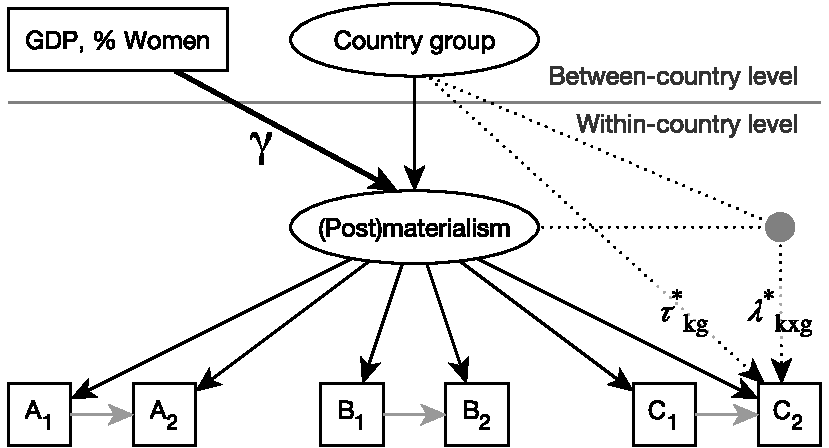
\includegraphics[width=0.6\textwidth]{figures/model}
	\caption{\label{fig:model}Graphical representation of 
	the multilevel latent class regression model for 
	(post)materialism measured by three partial ranking tasks. Observed variables are shown in rectangles while unobserved (``latent'') variables are shown in ellipses.	}
\end{figure}


The latent (post)materialism variable is measured by respondents' rankings of value priorities.
Each respondent in the 48 countries has ranked only their first and second choice on three ranking tasks A, B, and C (see Table \ref{tab:ranking-question}). We assume that each value priority has a particular ``utility'' \citep[p. 171]{luce1959individual,bockenholt2002comparison} dependent on the latent class variable  \citep[p. 172]{croon1989latent,bockenholt2002comparison}.  For example, for ranking task $A$ in country $c$, respondent $i$'s  choices for first and second place are modeled as
 \begin{equation}
	P(A_{1ic} = a_1, A_{2ic} = a_2 | X_{ic} = x) = 
		\frac{\exp(\tau_{a_1} + \lambda_{a_1 x})}{\sum_{k} \exp(\tau_{k} + \lambda_{k x})}
		\frac{\exp(\tau_{a_2} + \lambda_{a_2 x})}{\sum_{k \neq a_1}
			\exp(\tau_{k} + \lambda_{k x})},
				\label{eq:ranking}
\end{equation}
Crucially, the choice for second place, $A_{2ic}$, is modeled while excluding the alternative already chosen for first place, $A_{1ic}$. In other words, we model a sequential ranking process in which first place is chosen from all options, then second place is chosen from the remaining options. This dependency intrinsic to ranking tasks makes the model used here different from standard models for categorical dependent variables.
The measurement model for (post)materialism is shown in the bottom part of Figure \ref{fig:model}, using gray arrows to indicate that the choice for second place is modeled conditionally upon that for first place.

%As shown in Section \ref{sec:invariance}, Equation \ref{eq:ranking} is a full measurement invariance model: it excludes potential  direct main effects and direct interaction effects of the grouping variable. Instead of considering main and interaction effects from the countries directly, we consider these for the country random effects ($G$)  \citep[see][]{dejong2007relaxing,fox2011random,jak2014measurement}.
Measurement invariance violations could be parameterized by extending Equation  \ref{eq:ranking} to include country group class ($g$) effects:
\begin{equation}
P(A_{1ic} = a_1, A_{2ic} = a_2 | X_{ic} = x) = 
		\frac{\exp(\tau_{a_1} + \lambda_{a_1 x} + 
		\delta_{a_1 g} + \delta^{*}_{a_1 x g})}{\sum_{k} \exp(\tau_{k} + \lambda_{k x} + 
		\delta_{k g} + \delta^{*}_{k x g})}
		\ldots
			\label{eq:loglin-measurement-noninvariant}
\end{equation}
The base invariance model in Equation \ref{eq:ranking} can be seen as fixing the direct main effects $\delta_{k g} = 0$  and direct interaction effects $\delta^{*}_{k x g} = 0$. Figure \ref{fig:model}  shows an example for the second ranking of Set C ($C_2$) as the dotted main effect and interaction effects. In line with Section \ref{sec:invariance}, we now investigate whether the possible misspecifications in the measurement invariance model, $\delta_{k g} \neq 0$ and $\delta^{*}_{k x g} \neq 0$, substantially affect the parameters of interest $\gamma_{mx}$ using EPC-interest for categorical data.


The full measurement invariance model  including parameters of interest $\gamma_{mx}$ was estimated using Latent GOLD 5.  Following \citet{moors2007heterogeneity}, we select three  classes for both the latent ``(post)materialism'' variable and the country group class variable, $T = S = 3$. For BIC values and the rationale behind these choices, please see Appendix \ref{app:bic}. Since class selection is not the focus of this example analysis, we will not discuss it here further. 

After estimating the full invariance model, we calculated the $\da{}$ for the $\delta$ and $\delta^*$ parameters, of which our three-class model has four: two for each of the two independent variables. Measurement invariance violations can potentially take the form of 6 direct main effects ($\delta_{j k g}$) and 12 direct interaction effects ($\delta^{*}_{j k x g}$) for each of the three ranking tasks, totaling 54 possible misspecifications in the full invariance model. These misspecifications are strongly correlated and should not be considered separately. Rather, we consider the probable impact of freeing the direct main effects for each ranking task separately and of freeing the  direct interactions for each ranking task separately. Thus, rather than consider the direct and interaction effects for each of the 48 countries on each of the three unique categories of each of the three ranking tasks, making for $5076$ potential $\da{}$ values, we evaluate direct effects of the country group random effect and consider their impact jointly for strongly correlated misspecifications, reducing the problem to 24 $\da{}$ values of interest.


\begin{table}\begin{small}
	\caption{Full invariance multilevel latent class model: parameter estimates of interest with standard errors, and  $\da{}$ when freeing each of six sets of possible misspecifications. \label{tab:epc-interest-model1}}
	\begin{tabular}{lrrrrrrrrrrr}
	\hline
		&&&&&\multicolumn{7}{c}{EPC-interest for...}\\
	&&&&&\multicolumn{3}{c}{$\delta_{j k g}$} && \multicolumn{3}{c}{$\delta^{*}_{j k x g}$}\\
			\hline
		&&\multicolumn{2}{c}{Estimates $\hat{\gamma_{mx}}$}&&\multicolumn{3}{c}{Ranking task} && \multicolumn{3}{c}{Ranking task}\\
\cline{3-4}\cline{6-8}\cline{10-12}
			&	&	Est.&	s.e.&	&	1  &	2  &	3  &&	  1&	2 &	3\\
				\hline
Class	1&	GDP&	-0.035&	(0.007)&	&	-0.013&	0.021&	-0.002&&	\textbf{0.073}&	\textbf{0.252}&	0.005\\
Class	2&	GDP&	-0.198&	(0.012)&	&	-0.018&	-0.035&	0.015&&	-0.163&	-0.058&	0.002\\
\\
Class	1&	Women&	0.013&	(0.001)&	&	-0.006&	0.002&	0.000&&	-0.003&	0.029&	0.002\\
Class	2&	Women&	-0.037&	(0.001)&	&	0.007&	-0.003&	0.002&&	-0.006&	-0.013&	0.002\\
	\hline
\end{tabular}
\end{small}\end{table}

Table \ref{tab:epc-interest-model1} shows these 24 $\da{}$ values together with the parameter estimates from the full invariance model. The $\da{}$ values estimate the change from the current estimates of interest after freeing the direct main effects ($\delta_{jkg}$) or interaction effects ($\delta^*_{jkg}$). In the full invariance model, Class 1 corresponds to a ``postmaterialism'' class. The estimate -0.035 (s.e. 0.007) shown in Table \ref{tab:epc-interest-model1} would therefore suggest that more prosperous nations tend to be less postmaterialist. This directly contradicts the theory of \citet{inglehart2010changing}.

Since the theory specifies only that certain coefficients should be positive or negative, the key focus of substantive interest is whether misspecifications in the invariance model can potentially change the sign of a parameter of interest. In Table \ref{tab:epc-interest-model1}, we therefore look for $\da{}$ values that, when added to the estimates in column 3, would change the sign of those estimates. It can be seen in the Table that two such $\da{}$ are indeed present, namely the direct interaction effect of the country group class with the postmaterialism class on ranking tasks 1 and 2.  This means that the attribute parameters that define the classes for these two tasks differ over country groups, and that after accounting for these differences the effect of GDP on postmaterialism is estimated to be positive rather than negative. This set of misspecifications is thus of substantive interest and should be amended in the model. 

\begin{table}\begin{small}
	\caption{
	Partially invariant  multilevel latent class model: parameter estimates of interest with standard errors, and  $\da{}$ when freeing each of six sets of possible misspecifications. 
	\label{tab:epc-interest-model2}}
	\begin{tabular}{lrrrrrrrrrrr}
	\hline
		&&&&&\multicolumn{7}{c}{EPC-interest for non-invariance of...}\\
%		&&\multicolumn{2}{c}{Estimates}&&\multicolumn{3}{c}{Set} && \multicolumn{3}{c}{Set}\\
	&&&&&\multicolumn{3}{c}{$\delta_{k g}$} && \multicolumn{3}{c}{$\delta^{*}_{k x g}$}\\
			\hline
		&&\multicolumn{2}{c}{Estimates $\hat{\gamma}_{mx}$}&&\multicolumn{3}{c}{Ranking task} && \multicolumn{3}{c}{Ranking task}\\
\cline{3-4}\cline{6-8}\cline{10-12}
			&	&	Est.&	s.e.&	&	1  &	2  &	3  &&	  1&	2 &	3\\
				\hline
Class 1&	GDP&	-0.127&	(0.008)&	&	-0.015&	-0.003&	0.002&&	&	&	0.097\\
Class 2&	GDP&	0.057&	(0.011)&	&	-0.043&	-0.013&	0.002&&	&	&	0.161\\
\\
Class 	1&	Women&	0.008&	(0.001)&	&	-0.002&	0.000&	0.002&	&&	&	0.001\\
Class 	2&	Women&	0.020&	(0.001)&	&	-0.007&	-0.001&	0.002&	&&	&	0.007\\
\hline
	\end{tabular}
\end{small}\end{table}

Following the common practice of partial invariance models, we free these two sets of measurement invariance violations, allowing for differences in the parameters of ranking tasks 1 and 2 across country groups. Table \ref{tab:epc-interest-model2} shows the substantive parameter estimates and $\da{}$ interest values for the resulting partial invariance model. The likelihood ratio test of improvement in model fit is highly significant ($\chi^2_{\text{df} = 28} = 24607$). Moreover, the substantive  regression coefficient for the effect of GDP on the postmaterialism class (Class 2 in Table \ref{tab:epc-interest-model2}), is indeed positive after freeing the detected misspecifications. Re-calculating $\da{}$ values for the remaining possible misspecifications reveals that none of the possible misspecifications in this partial invariance model has the potential to change the substantive conclusions. We therefore conclude that the partial invariance model fits ``approximately'', since none of the substantive conclusions based on it are threatened by measurement invariance violations.

\bigskip
This section demonstrated the use of the EPC-interest for measurement invariance testing in a more complex example. A violation of measurement invariance was detected that could reverse the conclusions of substantive interest. After accounting for this violation, no further such violations are detected. 

\pagebreak

\section{Discussion and conclusion}
\label{sec:discussion}


Whenever groups are compared, measurement invariance is a concern. Particularly, it should be verified that substantive conclusions of interest are uncontaminated by possible cross-group differences in measurement. The ``expected parameter change in the parameter of interest'' or EPC-interest, a measure introduced by \citet{Oberski:WP:EPC-interest} for this purpose in the context of linear structural equation models, was extended in this paper  to categorical observed and latent variables as well as rankings and other types of data often encountered in the social sciences. 

The EPC-interest for categorical data is an approximation of the change in the parameters of substantive interest that we can expect to observe if a particular violation of measurement invariance were freed. A small simulation study showed that this approximation works well when the misspecification is moderate, and overestimates the bias somewhat when it is extreme. In this case, EPC-interest still indicates the most important violations of measurement invariance but the researcher may wish to verify that the expected parameter change is close to the actually observed change. 

Two example applications of categorical data latent variable models demonstrated the utility of the EPC-interest. The first application formulated a simple IRT-type ``ideal point'' model for US senators' votes, modeling their latent ideology as a function of party membership to estimate polarization in the 90th US Senate. After fitting the full invariance model, EPC-interest detected one violation of measurement invariance that substantially reduced the estimated polarization and made the ideal point estimates for some Republican senators considerably more liberal. The second example application looked at the relationship between latent (post)materialism on the one hand and, on the other, log-GDP per capita and the percentage of women in parliament using data from  67,568 respondents in 48 countries. A violation of measurement invariance existed that, when unaccounted for, could reverse substantive conclusions. The $\da{}$ allowed us to detect this problem and account for those violations of assumptions that were indeed influential on the substantive conclusions of interest.

We suggest to use the EPC-interest or other sensitivity analyses to evaluate measurement invariance as we did in the examples discussed above: start from a model that assumes measurement invariance, and evaluate the impact of these restrictions on the conclusions of interest. The entire resulting sequence of models should be reported so readers can reproduce the results and decide whether they agree that violations removed could be judged as substantively ``large'' and those left in the model as ``small''. An example of such a judgment, given in the application, is that a positive effect can be changed to a negative one or vice versa; in other applications, different criteria will be relevant.

Is it appropriate to free violations of measurement invariance where encountered\footnote{We thank an anonymous reviewer for raising this question.}? Freeing violations has long been standard practice in both the ``partial invariance'' literature \citep{byrne1989testing} and the DIF literature \citep{Holland:1993aa}, but there are situations in which it can be misleading--especially when the alternative model cannot identify further free parameters. An example is a model with only one invariance restriction so that the alternative model is simply the model with only \emph{a priori} reference indicators. In such cases the choice of indicator for which to free the parameters (i.e. the choice of reference indicator) cannot be determined based on model fit, and will often lead to opposite changes in the parameters of interest \citep{hancock2009tenuousness}. The EPC-interest can then still be used to investigate whether the conclusions are robust to violations of the assumptions. When they are not, however, there is no empirical basis on which to select a model. In other situations such as in the examples, however, the alternative model still imposes testable restrictions on the data. It then seems reasonable to proceed by freeing some restrictions while retaining others as is the common practice.

\bibliographystyle{pa}
\bibliography{/Users/daob/Dropbox/Bibliography/quality}

\clearpage\appendix

\section{Countries included in the study}
\label{sec:countries-included}
\singlespacing
\begin{tabular}{lllll}
\hline
ISO3 code & Country name&&ISO3 code & Country name\\
\hline
DZA&	Algeria		&&MAR&	Morocco		\\
ARM&	Armenia		&&NLD&	Netherlands, The		\\
AUS&	Australia	&&NZL&	New Zealand		\\
AZE&	Azerbaijan	&&NGA&	Nigeria		\\
BLR&	Belarus		&&PAK&	Pakistan		\\
CHL&	Chile		&&PER&	Peru		\\
CHN&	China		&&PHL&	Philippines		\\
COL&	Colombia	&&POL&	Poland		\\
CYP&	Cyprus		&&QAT&	Qatar		\\
ECU&	Ecuador		&&RUS&	Russian Federation	\\
EGY&	Egypt		&&RWA&	Rwanda		\\
EST&	Estonia		&&SGP&	Singapore			\\
DEU&	Germany		&&SVN&	Slovenia		\\
GHA&	Ghana		&&ESP&	Spain		\\
IRQ&	Iraq		&&SWE&	Sweden		\\
JPN&	Japan		&&TTO&	Trinidad and Tobago	\\
JOR&	Jordan		&&TUN&	Tunisia		\\
KAZ&	Kazakhstan	&&TUR&	Turkey			\\
KOR&	Korea, Republic of  &&UKR&	Ukraine		\\
KGZ&	Kyrgyzstan	&&USA&	United States		\\
LBN&	Lebanon		&&URY&	Uruguay		\\
LBY&	Libya		&&UZB&	Uzbekista�		\\
MYS&	Malaysia        &&YEM&	Yemen		\\
MEX&	Mexico          &&ZWE&	Zimbabwe		\\	
\hline
\end{tabular}
\doublespacing

\clearpage
\section{Latent GOLD Choice input for the full invariance model}\label{sec:LGinput}

The input below fits the full invariance model described in the paper, setting the possible violations of invariance to zero (0). The option ``score test'' in the output section (only available in Latent GOLD or Latent GOLD Choice $\geq5$) is then used to obtain the EPC-interest values.
Output and data for this example can be obtained from the online appendix at \url{http://}.

\begin{small}
\singlespace
\begin{verbatim}
options

   maxthreads=all;
   algorithm 
      tolerance=1e-008 emtolerance=0.01 
      emiterations=450 nriterations=70 ;
   startvalues
      seed=0 sets=30 tolerance=1e-005 iterations=50;
   bayes
      categorical=0 variances=0 latent=0 poisson=0;
   missing  excludeall;
   
   // NOTE: The option "scoretest" for output is used to obtain 
   //        the EPC-interest. This will also produce the score test ("MI")
   //        and EPC-self for the measurement invariance restriction
   
   output      
      parameters=effect  betaopts=wl standarderrors profile 
      probmeans=posterior
      frequencies bivariateresiduals estimatedvalues=regression
      predictionstatistics setprofile setprobmeans 
      iterationdetails scoretest ;

    // There are several ways of modeling ranking data using LG or LGChoice.
    //    The most computationally efficient is to use the so-called "3-file"
    //    setup in LGChoice employed here (see LGChoice manual). 

	choice = 3
   alternatives 'inglehart_wvs6_long.alt' quote = single
   id=alt
   choicesets 'inglehart_wvs6_long.set' quote = single
   id=set;

variables
   groupid country;
   caseid id;
   choicesetid set ;
   dependent value ranking;
   independent NY_GDP_PCAP_CD, SG_GEN_PARL_ZS;
   attribute int1 nominal, int2 nominal, int3 nominal;
   latent
      GClass  group nominal 3, 
      Class nominal 3;

equations
   // Group class intercept
   GClass <- 1 ;
   
   // Parameters of interest are logistic regression coefficients of 
   //        NY_GDP_PCAP_CD and SG_GEN_PARL_ZS.
   Class <- 1 + GClass + NY_GDP_PCAP_CD + SG_GEN_PARL_ZS;
   
   // Below, sets of possible violations of measurement invariance have been
   //        explicitly restricted to equal zero using "(0)". This will
   //        produce EPC-interest, EPC-self, and Score test output.
   value <- int1 + int2 + int3 + 
      int1 Class + int2 Class + int3 Class + 
      (0) int1 GClass + (0) int2 GClass + (0) int3 GClass + 
      (0) int1 Class  GClass + 
      (0) int2 Class GClass + 
      (0) int3 Class GClass ;
\end{verbatim}

\end{small}
\doublespacing

\clearpage
\section{Model selection for the example application}

\label{app:bic}

\begin{table}
\centering
\caption{Log-likelihood, number of parameters, and Bayesian Information Criterion (BIC) for models with different numbers of classes for the (post)materialism (within-country) and country group (between-country) latent class variables.\label{tab:loglikelihood-models}}
\begin{tabular}{rrrrrrrrr}
  \hline
 \multicolumn{4}{c}{(Post)materialism ($X$) classes, $|\{G\}| = 1$ } &  & \multicolumn{4}{c}{Country group ($G$) classes, $|\{X\}| = 3$} \\ 
\cline{1-4}\cline{6-9}
 \#Classes & Log-lik & \#Par & BIC($L^2$) &  & \#Classes & Log-lik & \#Par & BIC \\ 
  \hline
 1 & -460512.7 & 9 & -10346.1 &  & 1 & -447646.2 & 29 & 895616.3 \\ 
 2 & -449836.9 & 19 & -31586.2 &  & 2 & -444754.8 & 32 & 889867.0 \\ 
 3 & -447646.2 & 29 & -35855.8 &  & 3 & -443216.6 & 35 & 886824.1 \\ 
 4 & -446211.1 & 39 & -38614.4 &  & 4 & -442734.2 & 38 & 885892.8 \\ 
 5 & -445246.3 & 49 & -40432.4 &  & 5 & -442436.5 & 41 & 885330.9 \\ 
 6 & -444776.4 & 59 & -41260.3 &  & 6 & -442110.5 & 44 & 884712.3 \\ 
 7 & -444384.0 & 69 & -41933.4 &  & 7 & -441946.2 & 47 & 884417.3 \\ 
% 8 & -443959.8 & 79 & -42670.2 &  &  &  &  &  \\ 
% 9 & -443746.9 & 89 & -42984.3 &  &  &  &  &  \\ 
% 10 & -443470.8 & 99 & -43424.9 &  &  &  &  &  \\ 
% 11 & -443299.3 & 109 & -43656.2 &  &  &  &  &  \\ 
% 12 & -443086.0 & 119 & -43971.0 &  &  &  &  &  \\ 
% 13 & -442944.1 & 129 & -44143.3 &  &  &  &  &  \\ 
% 14 & -442837.3 & 139 & -44245.2 &  &  &  &  &  \\ 
   \hline
\end{tabular}
\end{table}

In choosing the number of classes for the (post)materialism (within-country) and country group (between-country) latent class variables, we follow the advice of \citet{lukovciene2010simultaneous} to first fix the number of country-group classes to unity and choose a number of within-country classes, subsequently fixing the number of within-country classes to this chosen number and determining the number of country-group (between-country) classes. The left-hand side of Table \ref{tab:loglikelihood-models} shows the log-likelihoods, number of parameters and Bayesian Information Criterion (BIC) values based on the $L^2$ for the model with one country-group class and an increasing number of (post)materialism classes. It can be seen that the BIC, which penalizes model complexity, decreases with each additional latent (post)materialism class. In fact, the BIC does not stop decreasing even when incrementing the number of classes to 14 (not shown in Table \ref{tab:loglikelihood-models} for brevity). 

In the literature on (post)materialism \citep[e.g.][]{inglehart2010changing}, the number of (post)materialism classes is typically fixed to three: ``postmaterialist'', ``materialist'', and ``mixed''. Clearly, using the WVS ranking tasks and imposing full invariance, many more qualitative (post)materialism classes can be distinguished than the traditional three classes. This corresponds to findings by \citet{moors2007heterogeneity}; however, these authors also argued that ``one can safely interpret the results (...) if adding another class does not result in important changes of the latent class weights for the other classes'' (p. 637). While this is a somewhat subjective criterion, the three-class solution found in the data does correspond to  the theoretical ``postmaterialist'', ``materialist'', and ``mixed'' classes, whose  parameters appear to change little in the models with a greater number of classes. Moreover, the greatest reduction in BIC seen in Table \ref{tab:loglikelihood-models} takes place when moving from a one-class to a two-class model, with relatively small improvements after three or more classes. We therefore follow the theoretical literature in selecting the three-class model.

While selecting the number of country-group classes, we find that the BIC improves little after three classes (right-hand side of Table \ref{tab:loglikelihood-models}), so that our initial full invariance model has three (post)materialism (within-country) and three country group (between-country) classes. 


\section{WVS ranking data model estimates}



Table \ref{tab:attribute-parameters} shows the sizes of the three (post)materialism classes (third row) as well as the ``attribute parameters'', i.e. each class's average log-utility. 
Thus, when reading each row horizontally, the class with the highest log-utility represents respondents who value that object highest. For example, priorities A.1, A.2, B.1, B.3, and C1 have the highest log-utilities in Class 1. Since all of these priorities are ``materialist'' (labeled ``M'' in Table \ref{tab:attribute-parameters}), we also labeled Class 1 ``materialist''. A caveat with this label is that the materialist priorities that are most strongly related to this class also happen to be the first item in each set, so that a primacy effect may play a role here as well.  Class 2 is labeled ``postmaterialist'' because it has the highest log-utilities for all of the postmaterialist priorities (labeled ``P'' in Table \ref{tab:attribute-parameters}), with the exception of A.4. Preferences in the third class appear to be for the most part in-between those of Classes 1 and 2. At the same time, however, this class has the highest log-utilities for A.4 (a ``postmaterialist'' object) and C.4 (a ``materialist'' object). For this reason we apply the label ``mixed'' to Class 3.

\begin{table}\centering
	\caption{\label{tab:attribute-parameters} Estimated log-utilities under the 
		final model. In each row, the highest log-utility has been printed in \textbf{bold face} to facilitate interpretation of the classes.}
	\begin{tabular}{lllrrr}
	\hline
			&&&	Class 1	&	Class 2	&	Class 3\\
			&&Class label& ``Materialist'' & ``Postmater.'' & ``Mixed''\\
&& Class size & 0.569 & 0.213 & 0.218\\
&& (s.e.)				& (0.0114)	&	(0.0179)	&	(0.0280)\\
				\hline
\multicolumn{3}{l}{Set A}\\
& M & 1. Economic growth	&	\textbf{2.1102}	&	0.4837	&	0.4156\\
& M & 2. Strong defense	&	\textbf{-0.5285}	&	-1.4984	&	-0.9249\\
& P & 3. More say	&	-0.5519	&	\textbf{1.4683}	&	0.4643\\
& P & 4. More beauty	&	-1.0298	&	-0.4536	&	\textbf{0.0449}\\
\multicolumn{3}{l}{Set B}\\
& M & 1. Order in the nation	&	\textbf{1.0016}	&	-0.5898	&	0.0435\\
& P & 2. More say	&	-0.4592	&	\textbf{0.6902}	&	-0.2763\\
& M & 3. Rising prices	&	\textbf{0.4281}	&	-0.2269	&	0.3719\\
& P & 4. Freedom of speech	&	-0.9705	&	\textbf{0.1266}	&	-0.1390\\
\multicolumn{3}{l}{Set C}\\
& M & 1. Stable economy	&	\textbf{2.0086}	&	0.0789	&	0.1715\\
& P & 2. Humane society	&	-0.7919	&	\textbf{0.4450}	&	-0.0943\\
& P & 3. Ideas	&	-1.1402	&	\textbf{-0.0593}	&	-0.4550\\
& M & 4. Fight crime	&	-0.0765	&	-0.4646	&	\textbf{0.3778}\\
	\hline
	\end{tabular}
\end{table}




\section{Derivation of the EPC-interest}


The derivation of the $\da{}$ given in Equation \ref{eq:epc-interest} starts from the full invariance solution. We then find a hypothetical new  maximum of the likelihood by setting the gradient of a Taylor expansion of the likelihood around the full invariance solution to zero:
\begin{equation}
 \frac{\partial L(\param, \bpsi)}{\partial \vm{\vartheta}}= \vm{0} = 
	\left( \begin{array}{cc}
	\frac{\partial L(\param, \bpsi) }{ \partial \param}|_{\param=\that}\\
	\frac{\partial L(\param, \bpsi) }{ \partial \bpsi}|_{\param=\that}\\
	\end{array} \right)  + 
%	\left(\frac{\partial^2 L(\param, \bpsi) }{ \partial \vm{\vartheta}^\prime \partial \vm{\vartheta}} \right)
	\left( \begin{array}{cc}
		\hat{\vm{H}}_{\param\param} & \hat{\vm{H}}_{\bpsi\param}\\
		\hat{\vm{H}}_{\bpsi\param} & \hat{\vm{H}}_{\bpsi\bpsi}\\
	\end{array} \right)  
		\left( \begin{array}{cc}
		\param - \that\\
		\bpsi - \hat{\bpsi}
	\end{array} \right)+
O(\vm{\delta}^\prime\vm{\delta}).
	\label{eq:gradient}
\end{equation}
A similar device was used to derive the so-called ``modification index'' or ``score test'' for the significance of the hypothesis $\bpsi = \vm{0}$ by \citet[p. 373]{sorbom1989model}.
Equation \ref{eq:epc-interest}  follows directly by noting that $( \partial L(\param, \bpsi) / \partial \param ) |_{\param=\that} = \vm{0}$ and applying the standard linear algebra result on the inverse of a partitioned matrix $\left(\hat{\vm{H}}^{-1}\right)_{\param\bpsi} = 	- \hat{\vm{H}}^{-1}_{\param\param} \hat{\vm{H}}_{\param\bpsi}\vm{D}^{-1}$ \citep[e.g.][p. 12]{magnus2007matrix}.


\end{document}
